\documentclass[conference]{IEEEtran}
\IEEEoverridecommandlockouts
% The preceding line is only needed to identify funding in the first footnote. If that is unneeded, please comment it out.
\usepackage{cite}
\usepackage{amsmath,amssymb,amsfonts}
\usepackage{algorithmic}
\usepackage{graphicx}
\usepackage{textcomp}
\usepackage{xcolor}
\usepackage{placeins}
\usepackage[hidelinks]{hyperref}
\usepackage{float}
\usepackage{subcaption}
\def\BibTeX{{\rm B\kern-.05em{\sc i\kern-.025em b}\kern-.08em
    T\kern-.1667em\lower.7ex\hbox{E}\kern-.125emX}}
\begin{document}

\title{Redes Neurais Convolucionais}

\author{\IEEEauthorblockN{Arthur Abrahão Santos Barbosa}
\IEEEauthorblockA{\textit{Universidade Federal de Pernambuco} \\
\textit{Centro de Informática}\\
Pernambuco, Brasil \\
aasb2@cin.ufpe.br}
\and
\IEEEauthorblockN{Filipe Samuel da Silva}
\IEEEauthorblockA{\textit{Universidade Federal de Pernambuco} \\
\textit{Centro de Informática}\\
Pernambuco, Brasil \\
fss8@cin.ufpe.br}

}

\maketitle





\section{Objetivos}

\subsection{Objetivo Geral}

Desnvolver um Classificador Multiclasse que reconheça as imagens do dataset CIFAR100 \cite{dataset}. 
\subsection{Objetivos Específicos}
\begin{itemize}
\item Compreender a implementação de uma Rede Neural Convolucional
\item Demonstrar a Importância do Aprendizado Profundo e suas aplicações
\item Demonstrar a eficiência de três arquiteturas importantes para a história do Deep Learning
\end{itemize}
\section{Justificativa}
Este projeto foi escolhido com base no fato deste dataset ser bastante usado para testar redes neurais com imagens coloridas, 
e pelo fato de ter uma divisão bastante equilibrada dos dados.\cite{dataset}.


Sua função é verificar a qual das classes pertence uma imagem de tamanho 32x32.

\section{Base de Dados}

O dataset usado durante o projeto é o CIFAR-100.
Ele tem 100 classes contendo 600 imagens cada, totalizando 60.000 imagens.
Das 600 imagens que cada classe possui 100 delas são separadas para teste e 500 delas para treino.
As 100 classes do dataset estão agrupadas em 20 super classes do seguinte modo\cite{dataset}:

\begin{itemize}
    \item \textbf{aquatic mammals:} 	beaver, dolphin, otter, seal, whale
    \item \textbf{fish:} 	aquarium fish, flatfish, ray, shark, trout
    \item \textbf{flowers:} 	orchids, poppies, roses, sunflowers, tulips
    \item \textbf{food containers:} 	bottles, bowls, cans, cups, plates
    \item \textbf{fruit and vegetables:} 	apples, mushrooms, oranges, pears, sweet peppers
    \item \textbf{household electrical devices:} 	clock, computer keyboard, lamp, telephone, television
    \item \textbf{household furniture:} 	bed, chair, couch, table, wardrobe
    \item \textbf{insects:} 	bee, beetle, butterfly, caterpillar, cockroach
    \item \textbf{large carnivores:} 	bear, leopard, lion, tiger, wolf
    \item \textbf{large man-made outdoor things:} 	bridge, castle, house, road, skyscraper
    \item \textbf{large natural outdoor scenes:} 	cloud, forest, mountain, plain, sea
    \item \textbf{large omnivores and herbivores:} 	camel, cattle, chimpanzee, elephant, kangaroo
    \item \textbf{medium-sized mammals:} 	fox, porcupine, possum, raccoon, skunk
    \item \textbf{non-insect invertebrates:} 	crab, lobster, snail, spider, worm
    \item \textbf{people:} 	baby, boy, girl, man, woman
    \item \textbf{reptiles:} 	crocodile, dinosaur, lizard, snake, turtle
    \item \textbf{small mammals:} 	hamster, mouse, rabbit, shrew, squirrel
    \item \textbf{trees:} 	maple, oak, palm, pine, willow
    \item \textbf{vehicles 1:} 	bicycle, bus, motorcycle, pickup truck, train
    \item \textbf{vehicles 2:}	lawn-mower, rocket, streetcar, tank, tractor

\end{itemize}
\cite{dataset}


\section{Análise Exploratória dos Dados}

\subsection{Quantidade de Imagens Por Classes}

Tanto o dataset de teste quanto o de treino são bastante equilibrados,
possuindo a mesma quantidade de imagens para cada classe:


\subsection{Descrição Estatística dos dados}

Porque os dados trabalhados são imagens em vez de tabelas,
é mais difícil descrevê-las estatisticamente.
Portanto as descrevemos do seguinte modo:

\subsubsection{Média das Imagens por Classe}

Um método possível de analisar as imagens estatisticamente
é cálcular o valor médio por pixel, e deste modo conseguir uma imagem média que
representaria a classe.

\begin{itemize}
\item Média da Imagens Não Normalizadas
\end{itemize}

\begin{figure}[H]
\centerline{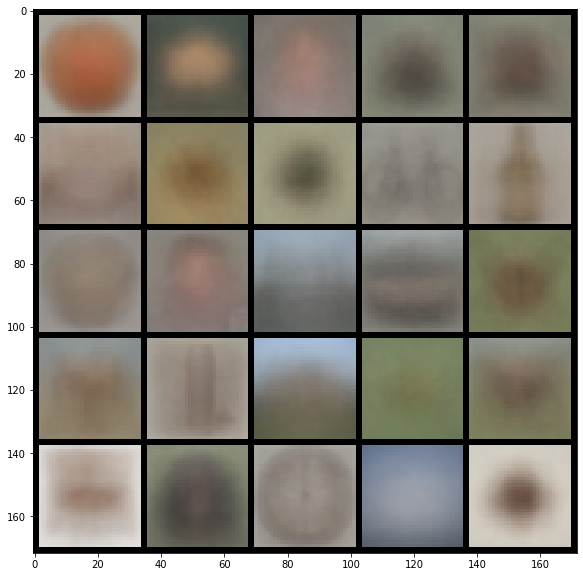
\includegraphics[width=0.4\textwidth]{Images/img_mean1.png}}
\caption{\label{fig:img_mean1}Da esquerda para a direita, de cima para a baixo: apple, aquarium\_fish, baby, bear, beaver, bed, bee, beetle, bicycle, bottle, bowl, boy, bridge, bus, butterfly, camel, can, castle, caterpillar, cattle, chair, chimpanzee, clock, cloud, cockroach}
\end{figure}

\begin{figure}[H]
\centerline{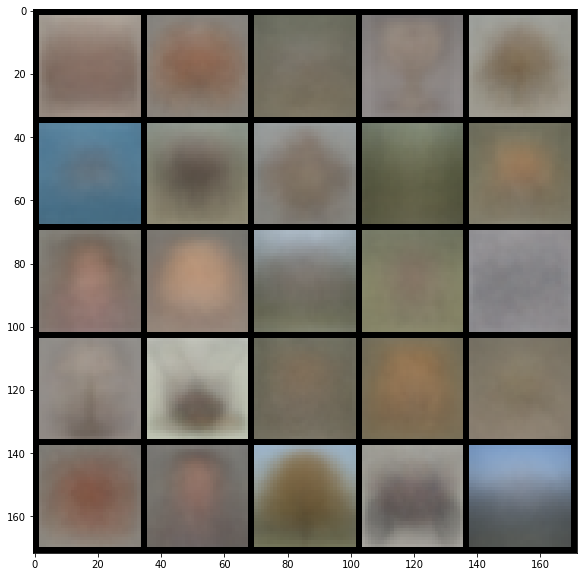
\includegraphics[width=0.4\textwidth]{Images/img_mean2.png}}
\caption{\label{fig:img_mean2}Da esquerda para a direita, de cima para a baixo: couch, crab, crocodile, cup, dinosaur, dolphin, elephant, flatfish, forest, fox, girl, hamster, house, kangaroo, keyboard, lamp, lawn\_mower, leopard, lion, lizard, lobster, man, maple\_tree, motorcycle, mountain}
\end{figure}

\begin{figure}[H]
\centerline{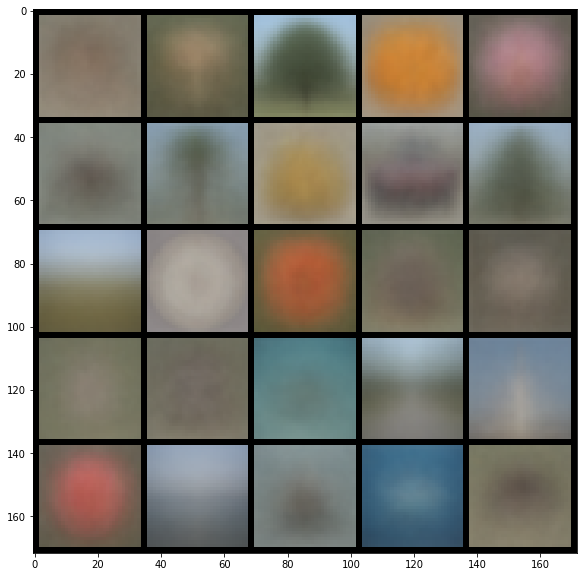
\includegraphics[width=0.4\textwidth]{Images/img_mean3.png}}
\caption{\label{fig:img_mean3}Da esquerda para a direita, de cima para a baixo: mouse, mushroom, oak\_tree, orange, orchid, otter, palm\_tree, pear, pickup\_truck, pine\_tree, plain, plate, poppy, porcupine, possum, rabbit, raccoon, ray, road, rocket, rose, sea, seal, shark, shrew}
\end{figure}

\begin{figure}[H]
\centerline{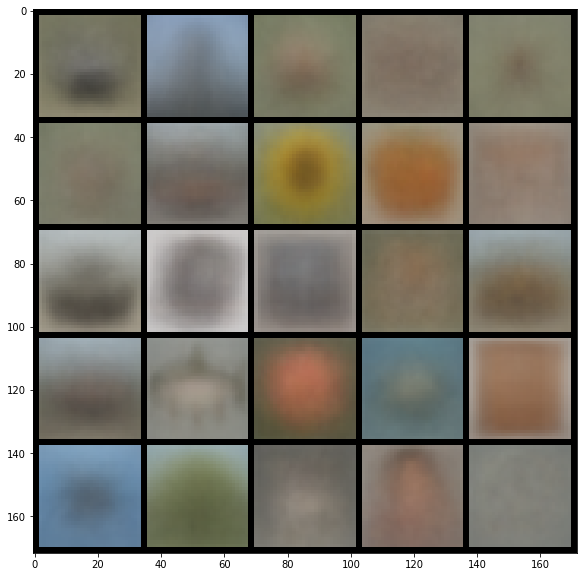
\includegraphics[width=0.4\textwidth]{Images/img_mean4.png}}
\caption{\label{fig:img_mean4}Da esquerda para a direita, de cima para a baixo: skunk, skyscraper, snail, snake, spider, squirrel, streetcar, sunflower, sweet\_pepper, table, tank, telephone, television, tiger, tractor, train, trout, tulip, turtle, wardrobe, whale, willow\_tree, wolf, woman, worm}
\end{figure}

\begin{itemize}
\item Média da Imagens Normalizadas
\end{itemize}

\begin{figure}[H]
\centerline{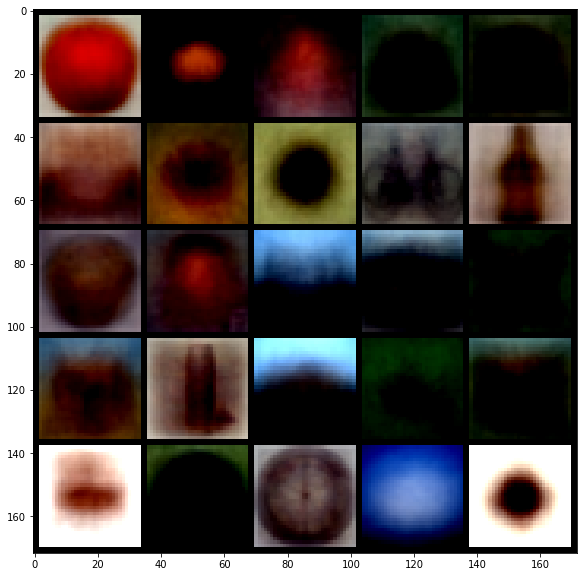
\includegraphics[width=0.4\textwidth]{Images/img_mean_norm1.png}}
\caption{\label{fig:img_mean_norm1}Da esquerda para a direita, de cima para a baixo: apple, aquarium\_fish, baby, bear, beaver, bed, bee, beetle, bicycle, bottle, bowl, boy, bridge, bus, butterfly, camel, can, castle, caterpillar, cattle, chair, chimpanzee, clock, cloud, cockroach}
\end{figure}

\begin{figure}[H]
\centerline{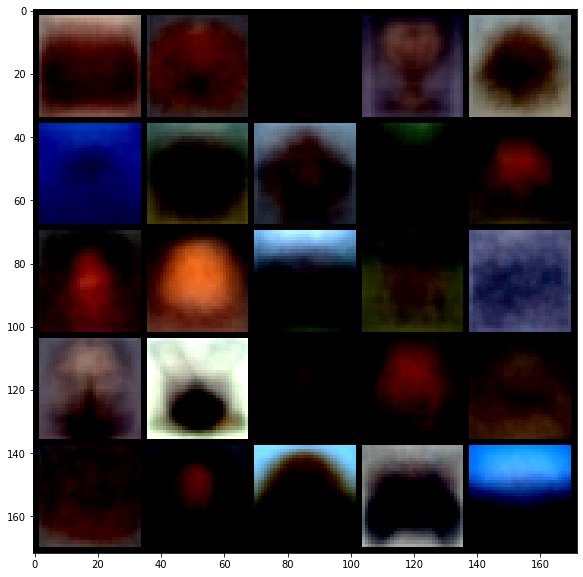
\includegraphics[width=0.4\textwidth]{Images/img_mean_norm2.png}}
\caption{\label{fig:img_mean_norm2}Da esquerda para a direita, de cima para a baixo: couch, crab, crocodile, cup, dinosaur, dolphin, elephant, flatfish, forest, fox, girl, hamster, house, kangaroo, keyboard, lamp, lawn\_mower, leopard, lion, lizard, lobster, man, maple\_tree, motorcycle, mountain}
\end{figure}

\begin{figure}[H]
\centerline{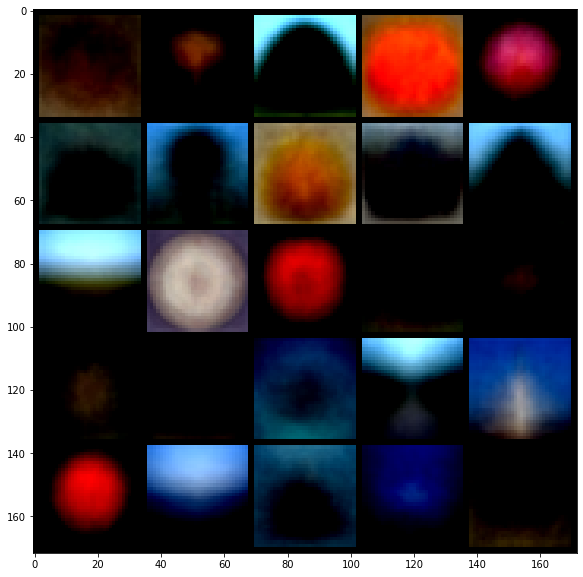
\includegraphics[width=0.4\textwidth]{Images/img_mean_norm3.png}}
\caption{\label{fig:img_mean_norm3}Da esquerda para a direita, de cima para a baixo: mouse, mushroom, oak\_tree, orange, orchid, otter, palm\_tree, pear, pickup\_truck, pine\_tree, plain, plate, poppy, porcupine, possum, rabbit, raccoon, ray, road, rocket, rose, sea, seal, shark, shrew}
\end{figure}

\begin{figure}[H]
\centerline{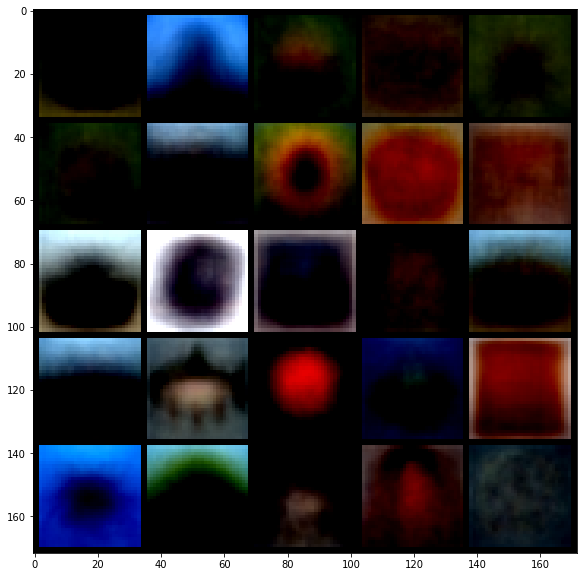
\includegraphics[width=0.4\textwidth]{Images/img_mean_norm4.png}}
\caption{\label{fig:img_mean_norm4}Da esquerda para a direita, de cima para a baixo: skunk, skyscraper, snail, snake, spider, squirrel, streetcar, sunflower, sweet\_pepper, table, tank, telephone, television, tiger, tractor, train, trout, tulip, turtle, wardrobe, whale, willow\_tree, wolf, woman, worm}
\end{figure}
    
%\subsection{Sobre o Projeto}
%Para montar o classificador foi necessário passar  pelas seguintes etapas:



\section{Sobre as Métricas Utilizadas}

\subsection{Precision}

Precision é a razão
    \begin{equation}
        \frac{A_c}{A_c + A_e}
    \end{equation}

    onde:

    \begin{itemize}
    \item $A_c$ é o número de amostras corretamente classificadas de uma determinada classe.
    \item $A_e$ é o número de amostras  erroneamente classificadas como sendo desta determinada classe.
    \end{itemize}

    Precision é intuitivamente a habilidade do classificador não marcar como pertencente a uma classe uma amostra que não pertence a esta. O melhor valor de Precision é 1 e o pior é zero.
    \cite{b7}
\subsection{Accuracy} 

Accuracy é a fração de amostras preditas corretamente, e é dada pela seguinte fórmula:

\begin{equation}
    \frac{\sum\limits_{1}^{n}A_c}{\sum\limits_{1}^{n}A_t}
\end{equation}




onde:
\begin{itemize}
    \item $n$ é o número de classes
    \item $A_c$ é o número de amostras corretamente classificadas de uma determinada classe.
    \item $A_t$ é o número de amostras que pertencem a uma determinada classe
\end{itemize}

\cite{b8}
\subsection{Recall-Score}
O Recall Score é a razão:

    \begin{equation}
        \frac{A_c}{A_t}
    \end{equation}
    onde:
    \begin{itemize}
        \item $A_c$ é o número de amostras classificadas corretamente de uma determinada classe
        \item $A_t$ é o número de amostras que pertencem a esta classe
    \end{itemize}
    O Recall Score é intuitivamente a habilidade do classificador de encontrar todas as amostras pertencentes a uma classe especifica. O melhor valor do Recall Score é 1 e o pior valor é 0.
    \cite{b6}

\subsection{F1-Score}
O F1 Score pode ser interpretado como a média ponderada da precisão e recall. O melhor valor que o  F1 score pode alcançar é 1, o pior é 0. A contribuição relativa da precisão e recall para o F1 score são iguais. A fórmula para o F1 score é:
\begin{equation}
    F1 = \frac{2\cdot(precision\cdot recall)}{precision + recall}
\end{equation}
\cite{b2}
\subsection{Confusion Matrix}
No caso de classificação multiclasse, uma confusion matrix é dividida em NxN categorias(onde N é o número de classes do problema), cada uma apresentando a quantidade de amostras que se encaixam nesta.
A diagonal do meio representa a quantidade de amostras classificadas corretamente e as demais seções da matriz demonstram o número de amostras classificados erroneamente, a quais classes eles pertencem e em quais classes eles foram classificados.

\cite{metrics}




\section{Redes Neurais Convolucionais}


\subsection{O Nosso Modelo}
\subsection{AlexNet}

\subsection{GoogLeNet}




\section{Experimentos}

%\subsection{Experimentos Iniciais}

\subsection{CIFAR10}


\subsection{Similaridade de Pixel}

Baseado na abordagem do fastai \cite{howard2020deep}
iremos criar um modelo básico que não utiliza aprendizado de máquina, 
para ter uma precisão como base para verificar o desempenho dos próximos modelos.
 Esse método basicamente cálcula uma imagem média para cada classe do conjunto de treino, 
 esta imagem média é basicamente uma imagem formada pela média de cada pixel das imagens de uma classe.

Para fazer a predição esta arquitetura basicamente cálcula a distância de uma imagem a imagem média,
e escolhe a classe com a menor distância.
Podemos usar o erro quadrático médio ou o valor absoluto das diferenças como valor da distância total entre uma imagem e a média da sua classe.

Porém, ao contrário da abordagem original do fastai para o dataset mnist com apenas duas classes com imagens em preto e branco, 
que teve uma 'accuracy' razoável com este método, temos que a 'accuracy' que tivemos com o CIFAR 100 que possui muito mais classes,
e imagens coloridas, não é melhor do que selecionarmos uma classe ao acaso.

\subsection{Treinando os Modelos}

\subsection{Apenas um Epoch}

\subsection{Imagens em Grayscale}

\subsection{Limitando os Dados}


\subsection{Sem Normalização e sem Data Augmentation}





%\subsection{Modelos Pré-Treinados}

\section{Análise dos Resultados}




\section{Conclusões e Discussões}


\bibliography{mybib}
\nocite{*}
\bibliographystyle{IEEEtran}
\end{document}
